\documentclass[9pt]{beamer}
\usetheme[faculty=fi]{fibeamer}
\usepackage[T2A]{fontenc}
\usepackage[utf8]{inputenc}
\usepackage[
  main=ukrainian, %% By using `czech` or `slovak` as the main locale
                %% instead of `english`, you can typeset the
                %% presentation in either Czech or Slovak,
                %% respectively.
  english, russian %% The additional keys allow foreign texts to be
]{babel}        %% typeset as follows:
%%
%%   \begin{otherlanguage}{czech}   ... \end{otherlanguage}
%%   \begin{otherlanguage}{slovak}  ... \end{otherlanguage}
%%
%% These macros specify information about the presentation
\title{Криптосистеми на еліптичних кривих} %% that will be typeset on the
%\subtitle{Presentation Subtitle}
\subtitle{Lecture 7: Gentle intro to pairings}

\author{Грубіян Євген Олександрович}

%% These additional packages are used within the document:
\usepackage{ragged2e}  % `\justifying` text
\usepackage{booktabs}  % Tables
\usepackage{tabularx}
\usepackage{tikz}      % Diagrams
\usetikzlibrary{calc, shapes, backgrounds}
\usepackage{amsmath, amssymb}
\usepackage{url}       % `\url`s
\usepackage{listings}  % Code listings
\usepackage{wrapfig}
\frenchspacing
\begin{document}
  \frame{\maketitle}


  \begin{darkframes}
      
    \section{Light Frames}


\begin{frame}{Вступ до білінійного спарювання}
  \begin{itemize}
    \item Білінійні спарювання – це математичні функції, що перетворюють пару елементів з двох груп у елемент третьої групи при цьому мають властивості лінійності за обома аргументами.
    \item Вони широко використовуються в криптографії для побудови протоколів, наприклад протоколів з нульовим розголошенням, протоколів широкомовного шифрування, протоколів підпису, протоколів на основі ідентифікаторів та деяких конструкцій функціонального шифрування.
    \item Суттєва властивість білінійних спарювань – це їх лінійність щодо кожного аргументу, що дозволяє отримувати складні криптографічні конструкції, зокрема перевіряти деякі властивості в "шифрованому просторі" без розкриття аргументів.
    \item Спарювання - корисний інструмент для криптоаналізу, зокрема вони вирішують задачу DDH (Decisional Diffie-Hellman Problem): $DDH(P,[a]P, [b]P, [c]P) \xrightarrow{[c]P =^? [ab]P} \{T,F\}$
  \end{itemize}
\end{frame}

\begin{frame}{Визначення білінійного спарювання}
  Нехай \(G_1\), \(G_2\) та \(G_T\) – абелеві групи порядку $n$. При цьому $G_1, G_2$ - групи з аддитивною нотацією, $G_T$ - група з мультиплікативною нотацією. Відображення
  \[
  e : G_1 \times G_2 \to G_T
  \]
  називається \emph{білінійним спарюванням}, якщо вона задовольняє наступні властивості:
  \begin{enumerate}
    \item \textbf{Білінійність:} Для всіх $P_1, P_2 \in G_1, Q_1, Q_2 \in G_2$: 
    $$e(P_1 + P_2, Q_1) = e(P_1,Q_1)e(P_2,Q_1),\ e(P_1, Q_1+Q_2)=e(P_1,Q_1)e(P_1,Q_2) $$
    \item \textbf{Невиродженість:} Якщо \(P \neq \mathcal{O}\) (нейтральний елемент у \(G_1\)), то існує \(Q \in G_2\) такий, що \(e(P,Q) \neq 1\), і навпаки.
    \item \textbf{Обчислюваність:} Існує ефективний алгоритм обчислення \(e(P,Q)\) для будь-яких \(P \in G_1\) та \(Q \in G_2\).
  \end{enumerate}


\end{frame}

\begin{frame}{Визначення білінійного спарювання}
  Зазначимо що властивість 1 також можна сформулювати у вигляді: $\forall a,b \in \mathbb{Z}_n: e([a]P, [b]Q) = e(P,Q)^{ab}$

  Білінійні спарювання над еліптичними кривими - досить давній об'єкт, що досліджувався ще Андре Вейлем в 30х-40х роках XX століття, власне існує знамените однойменне спарювання, яке ми будемо розглядати. Проте до 80х років це радше була теоретична конструкція, оскільки алгоритмів які б ефективно (за поліноміальний час) обчислювали його не існувало. Перший алгоритм який дозволив ефективно обчислити спарювання Вейля був наведений Міллером у 1985р (https://crypto.stanford.edu/miller/miller.pdf), проте його робота не приймалась до публікації довгий час, аж допоки в 90х роках за допомогою спарювань не була розроблена ефективна атака (MOV) на диcкректний логарифм суперсингулярних (вважались найркащими на той час) кривих (звісно ж атака застосовується для всіх кривих які мають низький степінь вкладення).
\end{frame}
\begin{frame}{Приклади білінійних спарювань в математиці}
  \begin{enumerate}
    \item Функція $f:\mathbb{R} \times \mathbb{R} \to \mathbb{R},\ f(x, y) = 2^{xy}$ є білінійним спарюванням
      \item Нехай \(V\) — векторний простір над полем \(F\). Скалярний добуток:
  \[
  e(u,v)=u\cdot v=\sum_{i=1}^{n} u_i\,v_i,\quad \text{де } u,v\in V.
  \]
  є білінійним спарюванням $e: V \times V \to F$
  \item Нехай \(F\) — розширення поля \(K\). Функція сліду
  \[
  e(a,b)=\operatorname{Tr}_{F/K}(ab)
  \]
  визначає білінійне спарювання \(F \times F \to K\). Якщо розширення сепарабельне, це спарювання невироджене (для розширення $F_{p^n}$ слід це $\operatorname{Tr}_{F_{p^n}/F_p}(a) = \sum_{k=0}^{n-1} a^{p^k}$ )
  \item Спарювання Вейля на групі точок порядку $n$ еліптичної кривої $E/F_q$: $e_w:E[n] \times E[n] \to F_{q^m}$
  \end{enumerate}

\end{frame}

\begin{frame}{Степінь вкладення}
Нехай $E/F_q$ - деяка еліптична крива над полем $F_q$, яка містить підгрупу порядку $m$ (зазвичай велике просте число), при цьому $gcd(q,m) = 1$. Важливим елементом для визначення спарювання є степінь вкладення еліптичної кривої в мультиплікативну групу деякого розширення поля $F_q$.
    \begin{block}{Степінь вкладення еліптичної кривої $E/F_q$}
        Мінімальне значення $r$, таке що якщо $m | E(F_q)$, то $ m \vert q^r-1$ або ж еквівалентно $r=ord_{\mathbb{Z}_m^*}(q)$
    \end{block}
    Тобто степінь вкладення - це мінімальний ступінь розширення поля куди вкладається підгрупа точок порядку $m$. Інакше кажучи група $m$-коренів з одиниці $\mu_m$ вкладається в $\mu_m \subset F_{q^r}$.
    
    Наприклад степінь вкладення суперсингулярної кривої $E/F_p:y^2=x^3+x,\ p \equiv 3 \pmod 4$ дорівнює 2: $\#E(F_p)=p+1 \vert p^2 -1 $
\end{frame}

\begin{frame}{MOV-атака}
  Маємо $P,Q=[x]P \in E[m]$ - точки порядку $m$ еліптичної кривої $E/F_q$ з невеликим (зазвичай $r\le6$) степенем вкладення. Наша мета - обчисилити дискретний логарифм $x$ точки $Q$
  \begin{block}{MOV-атака на дискретний логарифм}
    Обчислити білінійне спарювання (Вейля)
      \[
      e_w : E[m] \times E[m] \to \mu_m \subset \mathbb{F}_{q^r}^*.
      \]
      для \(P\) і \(Q = [x]P\): \(e_w(P, Q)\). Завдяки білінійності маємо:
      \[
      e_w(P, Q) = e_w(P, [x]P) = e_w(P,P)^x.
      \]
      Тоді задача знаходження \(x\) зводиться до розв’язання дискретного логарифму у \(\mathbb{F}_{q^r}^*\), де вона є субекспоненційною, тобто не такою складною як в групі $E[m]$
  \end{block}
  Саме тому на практиці для класичних криптосистем на базі ECDLP обирають криві з високим стуменем вкладення (на щастя імовірність зустріти таку при випадковому виборі дуже висока)
\end{frame}

\begin{frame}{Інтуїція за дівізорами}
    Для того щоб визначити спарювання Вейля $e_w:E[m]\times E[m] \to \mu_m$ потрібно трохи повернутись до витоків теорії еліптичних кривих, а саме до алгебраїчної геометрії. Ключовим засобом аналізу алгебраїчних кривих є дівізори, які є свого роду засобом що кодує будь які раціональні функції використовуючи підрахунок їх полюсів та коренів, аналогічно до того як корені кодують поліноми (інтерполяція Лагранжа).

    Приклад: візьмемо раціональну функцію із афінного простору $\mathbb{A}^1$: $f(x)=\frac{x^5}{(x-3)^2}$, ця фунція має корінь кратності 5 в точці 0, а також полюс в точці 3 кратності 2. Тобто знаючи корені та полюси можна задати будь яку раціональну функцію або ж мероморфну функцію (узагальнення на комплекснозначні функції) за допомогою дівізора. В нашому прикладі - $div(f) = 5(0) - 2(3)$
\end{frame}

\begin{frame}{Раціональні функції на еліптичній кривій}
    \begin{block}{Поле раціональних функцій кривої E/K: $\overline{K}(E)$}
    Поле всіх функцій що можуть бути представленими як відношення двох поліномів $f(x,y) = g(x,y)/h(x,y)$ заданих над замиканням $\overline{K}$. При цьому для деякої точки  $P=(a,b) \in E$ значення функції в точці: $f(P)=g(a,b)/h(a,b)$
    \end{block}
    Порядком точки $P$ відносно функції $f$ називають число $ord_P(f) \in \mathbb{Z}$ що є різницею кратностей $P$ як кореня чисельника $g$ та знаменника $h$. Зазначимо що порядок може бути від'ємний якщо точка є полюсом функції $f$
\end{frame}
\begin{frame}{Вступ до теорії дівізорів}
  \begin{block}{Дівізор алгебраїчної кривої $E$}
      Формальна суми точок (в нашому випадку крива - це знайома нам еліптична крива):
      \[
      D = \sum_{P \in E} n_P\,(P),\quad n_P \in \mathbb{Z},
      \]
      де лише скінченна кількість коефіцієнтів \(n_P\) відмінна від нуля, тобто майже всі $n_P$ нульові за виключенням скінченої кількості.
      \end{block}
      \begin{itemize}
          
    \item \textbf{Степінь дівізора:} $deg(D) = \sum_{P \in E} n_P$
    \item \textbf{Носій дівізора:} $supp(D) = \{P \in E | n_P \neq 0\}$
    \item Дівізорами в теорії еліптичних кривих зручно описувати перетин кривої $E$ із кривою що задається деякою раціональною функцією $f$ (наприклад прямою) $div(f)=\sum_{P\in E} ord_P(f) (P)$
\end{itemize}
\end{frame}

\begin{frame}{Група дівізорів}
  Неважко побачити що всі дівізори деякої еліптичної кривої $E$ формують вільну абелеву групу $Div(E)$ за операцією додавання дівізорів: $$D_1 + D_2 = \sum_{P\in E} (n_{P}^{(1)} + n_{P}^{(2)})(P) $$
  нейтральний елемент - нульовий дівізор - $(0)$

  Неважко довести що множина дівізорів степеня 0 утворює підгрупу $Div^0(E) \subset Div(E)$
\end{frame}

\begin{frame}{Приклади дівізорів}
    \begin{center}
    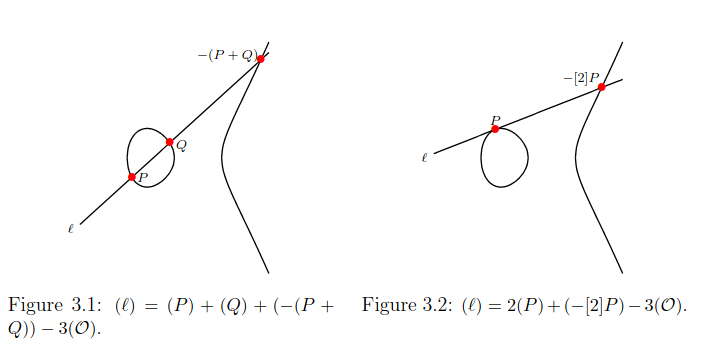
\includegraphics[width=0.8\textwidth]{resources/div.png}
    \end{center}
    Для січної прямої $\ell:f(x)=\lambda x +\nu$ що проходить через точки $P,Q$ її дівізор $div(f)=(\ell) = (P) + (Q) +(-(P+Q)) - 3(\mathcal{O})$.
    
    Для дотичної прямої в точці $P$ її дівізор: $(\ell) = 2(P) + (-[2]P) - 3(\mathcal{O})$

    З рівняння Вейєрштраса в проективних координатах підставивши рівняння прямої: $(\frac{\lambda X + \nu Z}{Z})^2 = (X/Z)^3 +aX/Z +b$ - виникає полюс порядку 3 в точці $\mathcal{O}_E =(0:1:0)$ в обох випадках. Також зазначимо що $deg((\ell))=0$ та $\sum_{P\in E} [n_P] P=\mathcal{O}_E$
\end{frame}

\begin{frame}{Головні дівізори}
    З попереднього прикладу видно що взявши раціональну функцію на кривій отримали що $deg(div(f))=0$, це не співпадіння, а частина значно ширшого результату з алгебраїчної геометрії де для будь якої раціональної функції на кривій її дівізор має нульовий степінь (але обернене твердження взагалі кажучи - невірне!). Таким чином можна ввести поняття головного дівізора
    \begin{block}{Головний (principial) дівізор}
        Дівізор $D$ називається головним, якщо існує деяка раціональна функція $f\in\overline{K}(E)$ що $D=(f)$
    \end{block}
    Множина головних дівізорів $Prin(E)$ є підгрупою $Div^0(E)$ (Якщо $(f), (g)$ - головні то дівізор $(f)+(g)=(fg)$ теж оскільки є дівізором добутку функцій $fg$. При цьому $(f)-(g)=(f/g)$ з чого маємо $(f)=(g) \iff (f/g)=0$ тобто $f,g$ відрізняються на константний множник). 

    
\end{frame}

\begin{frame}{Еквівалентні дівізори}
    Зазначимо що $D\in Prin(E) \iff (deg(D)=0) \land (\sum_{P\in E} [n_P] P = \mathcal{O}_E) $
    Таким чином маємо $Prin(E) \subset Div^0(E) \subset Div(E)$

    Головні дівізори корисні для подальшого визначення відношення еквівалентності на дівізорах $D_1\sim D_2 \iff \exists f \in \overline{K}(E): D_1-D_2=(f)$, тобто дівізори $D_1, D_2$ рівні з точністю до деякого головного дівізора.

    Це відношення є рефлексивним та симетричним (перевіряється досить легко) на $Div(E)$, але транзитивним лише на $Div^0(E)$, тобто $\sim \subseteq Div^0(E)^2$ - відношення еквівалентності на множині дівізорів нульового степеня.

    Таким чином $Div^0(E)/Prin(E)$ - фактор група дівізорів нульового степеня за модулем головних дівізорів $Pic^0(E)$ (ще називають якобіаном кривої або групою Пікарда).

    Відамий результат що $E(\overline{K}) \cong Pic^0(E)$, де ізморфізм задається $\phi(P) = (P)-(\mathcal{O}_E) $
    
\end{frame}

  \end{darkframes}




\end{document}
